\section{REST API}
\label{section:rest_api}
Vores API består af 3 dele:
\begin{itemize}
    \item Controllers der opsætter REST endpoints og konverterer data fra URLencoded / JSON til C\# objekter.
    \item Services’ der connecter til de forskellige databaser, og omskriver dataen til queries.
    \item Et databaselag bestående af 4 databaser som er opsat i cluster, hvis muligt.
\end{itemize}
På figur \ref{fig::api} har vi modelleret REST API’et med alle controllerens endpoints helt til venstre efterfulgt af alle services’, som håndterer dataen og sender det til den rigtige database. Alle endpoints går igennem “Create Log” servicen, som skriver til HBase med undtagelse af log controllerens egne endpoints. Udover log services har vi også en cache service, som består af 2 dele; en der henter en cache, hvis den findes og en der flusher cachen når en ny film eller serie, bliver lavet.

\begin{figure}[H]
    \centering
    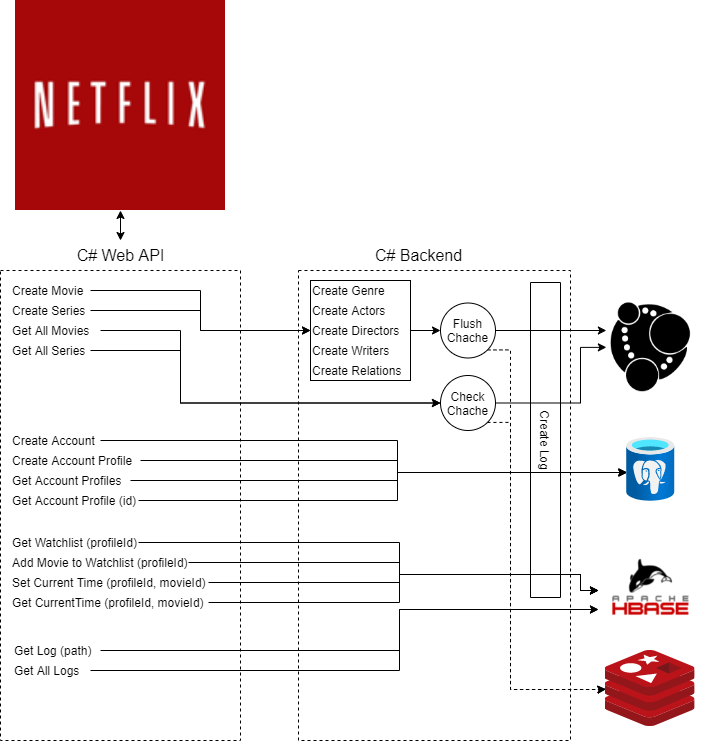
\includegraphics[scale=0.60]{api.png}
    \caption{REST API Model}
    \label{fig::api}
\end{figure}